\input{preamble}
\usepackage{tikz}
\usetikzlibrary{shapes,arrows}
\usepackage[normalem]{ulem}

\title{Online Behavioral Research Workshop}

\date[]{10 December 2015}

\begin{document}

\frame{\titlepage}

\frame{
\frametitle{Overview}
\begin{itemize}\itemsep1em
\item What is this course about?
\item Who are you?
\end{itemize}
}


\frame{
\frametitle{Learning Goals}

By the end of today you should be able to:

\begin{itemize}\itemsep1em
\item Describe logic of design-based and model-based representativeness
\item Evaluate the quality of a convenience sample
\item Design simple web forms using several tools
\item Evaluate trade-offs between client-side and server-side web technologies
\item Describe possible
\end{itemize}
}

\frame{\tableofcontents}


\frame{
\frametitle{Introductions}

\begin{itemize}\itemsep1em
\item Who are you?
\item What field are you from?
\end{itemize}
}

\frame{
\frametitle{About Me}

\begin{itemize}\itemsep1em
\item Assistant Professor at London School of Economics
\item PhD in Political Science from Northwestern University (2015)
\item Postdoc at Aarhus University 2012--2015
\item Interested in:
	\begin{itemize}
	\item Political psychology
	\item Survey--experimental methods
	\item Reproducible computational social science
	\end{itemize}
\end{itemize}
}


\frame{
\frametitle{How many of you have\dots}

\begin{itemize}\itemsep1em
\item<2-> taken a course on survey methods?
\item<3-> taken a course on experimental design?
\item<4-> written HTML markup before?
\item<5-> run a study on MTurk, Crowdflower, or another online platform?
\end{itemize}
}


\section{``The Gold Standard''}
\frame{\tableofcontents[currentsection]}


\frame{
\frametitle{``The Gold Standard''}

\begin{quote}\small
a population-based experiment uses survey sampling methods to produce a collection of experimental subjects that is representative of the target population of interest for a particular theory \dots the population represented by the sample should be representative of the population ot which the researcher intends to extend his or her findings. In population-based experiments, experimental subjects are randomly assigned to conditions by the researcher
\end{quote}

{\footnotesize p2. from Mutz, Diana. 2011. \textit{Popuation-Based Survey Experiments}. Princeton University Press.\par}

}

% design-based experimental inference
\frame{
	\frametitle{Causal Inference in Experiments I}
	\begin{itemize}\itemsep0.5em
    	\item<1-> Causal inference is a comparison of two \textit{potential outcomes}
    	\item<2-> A potential outcome is the value of the outcome (Y) for a given unit (i) after receiving a particular version/level/amount of the treatment (X)
    	\item<3-> Each unit has multiple \textit{potential} outcomes, but we only observe one of them
    	\item<4-> A \textit{causal effect} is the difference between two potential outcomes (e.g., $Y_{X=1} - Y_{X=0}$), all else constant
	\end{itemize}
}

\frame{
	\frametitle{Causal Inference in Experiments II}
	\begin{itemize}\itemsep2em
    	\item<1-> We cannot see individual-level causal effects
    	\item<2-> We can see \textit{average causal effects}
    		\begin{itemize}
        		\item<2-> Ex.: Average difference in participation between those with and without university degrees
    		\end{itemize}
    	\item<3-> We want to know: $TE_i = Y_{1i} - Y_{0i}$
	\end{itemize}
}

\frame{
	\frametitle{Causal Inference in Experiments III}
	\begin{itemize}\itemsep1em
		\item<1-> We want to know: $TE_i = Y_{1i} - Y_{0i}$
		\item<2-> We can average: $ATE = E[Y_{1i} - Y_{0i}] = E[Y_{1i}] - E[Y_{0i}]$
		\item<3-> But we still only see one potential outcome for each unit:\\ \vspace{1em}
    		$ATE_{naive} = E[Y_{1i} | X = 1] - E[Y_{0i} | X = 0]$
    	\item<4-> Is this what we want to know?
	\end{itemize}
}


\frame{
	\frametitle{Causal Inference in Experiments IV}
	\begin{itemize}\itemsep1em
	\item What we want and what we have:
		\begin{align}
		ATE & = E[Y_{1i}] - E[Y_{0i}] \\[1em]
		ATE_{naive} & = E[Y_{1i} | X = 1] - E[Y_{0i} | X = 0]
		\end{align}		
	\item<2-> Are the following statements true?\\
  		\begin{itemize}\itemsep1em
      		\item<2-> $E[Y_{1i}] = E[Y_{1i} | X = 1]$
      		\item<2-> $E[Y_{0i}] = E[Y_{0i} | X = 0]$
  		\end{itemize}
  	\item<3-> Not in general!
  	\end{itemize}
}

\frame{
	\frametitle{Causal Inference in Experiments V}
	\begin{itemize}\itemsep1em
    	\item Only true when both of the following hold:
    	\begin{align}
    	E[Y_{1i}] = E[Y_{1i} | X = 1] = E[Y_{1i} | X = 0]\\
    	E[Y_{0i}] = E[Y_{0i} | X = 1] = E[Y_{0i} | X = 0]
    	\end{align}
    	\item In that case, potential outcomes are \textit{independent} of treatment assignment
		\item If true, then:
    	\begin{align*}
    	ATE_{naive} & = E[Y_{1i} | X = 1] - E[Y_{0i} | X = 0] \tag{5}\\
    	& = E[Y_{1i}] - E[Y_{0i}]\\
    	& = ATE
    	\end{align*}
	\end{itemize}
}

\frame{
	\frametitle{Causal Inference in Experiments VI}
	\begin{itemize}\itemsep0.5em
    	\item This holds in experiments because of randomization\\
    		\begin{itemize}
        		\item Units differ only in what side of coin was up
        		\item Experiments randomly reveal potential outcomes
    		\end{itemize}
    	\item<2-> Matching attempts to eliminate those confounds, such that:
    	\begin{align*}
    	E[Y_{1i} | Z] = E[Y_{1i} | X = 1, Z] = E[Y_{1i} | X = 0, Z]\\
    	E[Y_{0i} | Z] = E[Y_{0i} | X = 1, Z] = E[Y_{0i} | X = 0, Z]
    	\end{align*}
	\end{itemize}
}

\frame{}


% design-based survey sampling

\frame{
	\frametitle{Inference Population}
	\begin{itemize}\itemsep2em
		\item We want to speak to a population
		\item But what population is it?
			\begin{itemize}
			\item<2-> A national population?
			\item<3-> Adults in Western, industrialized democracies?
			\item<4-> All human beings?
			\end{itemize}
	\end{itemize}
}


\frame{
	\frametitle{A Hypothetical Census}
	\begin{itemize}\itemsep2em
		\item Advantages
			\begin{itemize}
				\item<2-> Perfectly representative
				\item<2-> Sample statistics are population parameters
			\end{itemize}
		\item Disadvantages
			\begin{itemize}
				\item<3-> Costs
				\item<3-> Feasibility
				\item<3-> Need
			\end{itemize}		
	\end{itemize}
}


\frame{\frametitle{So, instead we sample!}}


\frame{
	\frametitle{Sampling Frames}
	\begin{itemize}\itemsep2em
		\item Enumeration (listing) of all units eligible for sample selection
		\item Two flavors:
			\begin{itemize}
				\item Random sample from an ordered list
				\item Systematic sampling from a randomized list
			\end{itemize}
		\item Building a sampling frame
			\begin{itemize}
				\item Combine existing lists
				\item Canvass/enumerate from scratch
			\end{itemize}
	\end{itemize}
}


\frame{
	\frametitle{Simple Random Sampling (SRS)}
	\begin{itemize}\itemsep2em
		\item Advantages
			\begin{itemize}
				\item Simplicity of sampling
				\item Simplicity of analysis
			\end{itemize}
		\item Disadvantages
			\begin{itemize}
				\item Need sampling frame and units without any structure
				\item Possibly expensive
			\end{itemize}
	\end{itemize}
}

\frame{
	\frametitle{Sample Estimates from an SRS}
	\begin{itemize}\itemsep1em
		\item Each unit in frame has equal probability of selection
		\item Sample statistics are unweighted
		\item Variances are easy to calculate
		\item Easy to calculate sample size need for a particular variance
	\end{itemize}
}

\frame{
	\frametitle{Sample mean}
	\begin{equation}
	\bar{y} = \frac{1}{n}\sum_{i=1}^{n}y_i
	\end{equation}
	where $y_i = $ value for a unit, and\\
	$n = $ sample size
	
	\begin{equation}
	SE_{\bar{y}} = \sqrt{(1-f)\frac{s^2}{n}}
	\end{equation}
	where $f = $ proportion of population sampled,\\
	$s^2 = $ sample element variance, and\\
	$n = $ sample size
}






\frame{
	\frametitle{Representativeness}
	
	What does it mean for a sample to be representative?
	
	\begin{itemize}\itemsep1em
		\item<2-> Census
		\item<3-> Simple random sampling
		\item<4-> Complex survey designs
		\item<5-> Quota sampling (common prior to the 1940s)
		\item<6-> Reweighting
		\item<7-> Others?
	\end{itemize}
}


% what kinds of representativeness do we care about?


% defining a target population
% question is: what do you want your survey



% defining your convenience sample
\frame{
	\frametitle{Convenience Samples}
	\begin{itemize}\itemsep1em
		\item<1-> What is a convenience sample?
		\item<2-> Different types:
			\begin{itemize}
				\item<3-> Passive/opt-in/``river sampling''
				\item<4-> Sample of convenience (not a sample per se)
					\begin{itemize}
					\item Email list
					\item Snowball sample
					\item Respondent-driven Sampling
					\end{itemize}
				\item<5-> Sample matching
				\item<6-> Online panels
			\end{itemize}
		\item<7-> ``Purposive'' samples (common in qualitative studies)
	\end{itemize}
}

% eligibility; duplication; recontacts



% response rates and biases
\frame{
\frametitle{Response Rates and Biases}
\begin{itemize}
\item The ``response rate'' is a traditional metric of survey quality
\item But, it's difficult to define in online/opt-in context
\item<2-> Bigger issue is ``reponse bias''
\end{itemize}
}




% question is how do they differ?


% suto


% sample characteristics

% attentiveness measures; satisficing; timing; response rates

% heterogeneous treatment effects

% induced value theory (swamping preferences)


\section{Web Questionnaires}
\frame{\tableofcontents[currentsection]}

% server-side versus client-side technologies
\frame{

When you navigate to a URL\dots

\begin{center}
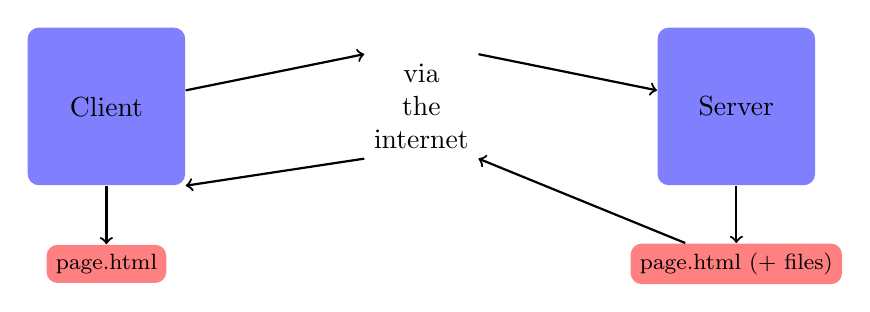
\begin{tikzpicture}
\draw<2-> node[fill=blue!50!white, rounded corners, minimum height=2cm, minimum width=2cm] (client) at (0,0) {Client};
\draw<2-> node[fill=blue!50!white, rounded corners, minimum height=2cm, minimum width=2cm] (server) at (8,0) {Server};
\draw<2-> node[align=center] (internet) at (4,0) {via\\the\\internet};
\draw<2->[thick, ->] (client) -- (internet.north west);
\draw<2->[thick, ->] (internet.north east)-- (server);

\draw<3-> node[fill=red!50!white, rounded corners, align=left] (page) at (8,-2) {{\footnotesize page.html (+ files)}};
\draw<3->[thick, ->] (server) -- (page);

\draw<4->[thick, ->] (page) -- (internet.south east);
\draw<4->[thick, ->] (internet.south west)-- (client.south east);

\draw<5-> node[fill=red!50!white, rounded corners, align=left] (page2) at (0,-2) {{\footnotesize page.html}};
\draw<5->[thick, ->] (client) -- (page2);

\end{tikzpicture}
\end{center}

\small

\begin{enumerate}
\item<2-> your browser sends an HTTP request to a server
\item<3-> the server processes the request and executes server-side code
\item<4-> the server replies with the contents of the page
\item<5-> your browser executes client-side 
\end{enumerate}
}



% what is a web survey?
\frame{

\frametitle{Questionnaires are client side}

A web page consists of four things:

\begin{itemize}
\item HTML describing content
\item Cascading style sheets (CSS) to style that content
\item Images or other multimedia content
\item Javascript code that makes a page dynamic
\end{itemize}

}



\begin{frame}[fragile]
\small
\begin{verbatim}
<html>
<head>
  <title>Survey</title>
</head>
<body>
  <form action="http://httpbin.org/post">
    <p>
      <label for="q1">Name: 
        <input type="text" name="q1" />
      </label>
    </p>
    <p><input type="submit"></p>
  </form>
</body>
</html>
\end{verbatim}
\end{frame}


% html
% html forms
%% <input type="radio" name="q2" value="1" />
%% <input type="checkbox" name="q2" value="1" />
%% <textarea name="open" rows="10" cols="30">
%% <select name="cars"><option value="volvo">Volvo</option></select>
%% <input type="hidden" />

% css

% javascript for randomized redirect
\begin{frame}[fragile]
\small
\begin{verbatim}
<html>
<head>
  <title>Redirect</title>
</head>
<body>
  <script>
  var u = new Array ();
  u[0] = "http://www.google.com";
  u[1] = "http://www.bing.com";
  u[2] = "http://www.yahoo.com";
  var i = Math.floor(u.length*Math.random());
  document.write("Redirecting to " + u[i]);
  window.location.replace(u[i]);
  </script>
</body>
</html>
\end{verbatim}
\end{frame}



% javascript for randomized display of a link
\begin{frame}[fragile]
\small
\begin{verbatim}
<html>
<head>
  <title>Redirect</title>
</head>
<body>
  <p>Please read the following:</p>
  <script>
  var u = new Array ();
  u[0] = "Treatment 1";
  u[1] = "Treatment 2";
  u[2] = "Treatment 3";
  var i = Math.floor(u.length*Math.random());
  document.write("<p><b>" + u[i] + "</b></p>");
  </script>
</body>
</html>
\end{verbatim}
\end{frame}


% javascript for youtube video presentation
\begin{frame}[fragile]
\tiny
\begin{verbatim}
<html>
<head>
  <title>Survey</title>
</head>
<body>
  <div id="player"></div>
  <script>
  var tag = document.createElement('script'); 
  tag.src = "https://www.youtube.com/iframe_api";
  var firstScriptTag = document.getElementsByTagName('script')[0];
  firstScriptTag.parentNode.insertBefore(tag, firstScriptTag);
  
  var player;
  function onYouTubeIframeAPIReady() {
    player = new YT.Player('player', {
      height: '390',
      width: '640',
      videoId: '0Bmhjf0rKe8',
      playerVars: {
        'controls': '0',
        'showinfo': '0',
        'rel': '0'
      },
      events: {
        'onReady': onPlayerReady
      }
    });
  }
  
  function onPlayerReady(event) {
    event.target.playVideo();
  }
  </script>
  
</body>
</html>
\end{verbatim}
\end{frame}





\frame{

\Large

If client-side is so cool\dots\\

\vspace{1em}

\dots why do we care about server-side technology?

}

\frame{


\begin{columns}[t]
\begin{column}{0.5\textwidth}
	\begin{block}{Client-Side}
		\begin{itemize}
		\item<2-> HTML (markup)
		\item<2-> CSS (styling)
		\item<2-> Javascript (scripting)
		\end{itemize}
	\end{block}
\end{column}
\begin{column}{0.5\textwidth}
	\begin{block}{Server-Side}
		\begin{itemize}
		\item<3-> Python, PHP, \dots
		\item<3-> Cookies
		\item<3-> Databases
		\end{itemize}
	\end{block}
\end{column}
\end{columns}

\vspace{1em}

\only<4->{We need a server to record a participant's behavior}

}




% Google Spreadsheet forms

\frame{
\frametitle{Web Questionnaires}
\begin{itemize}\itemsep1em
\item Google Spreadsheet Forms:\\
\url{https://www.google.co.uk/forms/about/}
\item 
\end{itemize}
}


\frame{
\frametitle{Google Consumer Surveys}
\begin{itemize}\itemsep1em
\item \url{http://www.google.com/insights/consumersurveys/home}
\item Features
	\begin{itemize}
	\item Cheap and fast
	\item Very limited functionality
	\item One-off questionnaires
	\item Great for pilot testing
	\end{itemize}
\end{itemize}
}


\frame{
\frametitle{Survey Monkey}
\begin{itemize}\itemsep1em
\item \url{https://www.surveymonkey.com/home/}
\item Features
	\begin{itemize}
	\item Free account
	\item Limited surveys and respondents
	\item No randomization in free account
	\item Nice respondent management tools
	\end{itemize}
\end{itemize}
}
% show off collectors and panel management


\frame{
\frametitle{Qualtrics}
\begin{itemize}\itemsep1em
\item \url{https://www.qualtrics.com/login/}
\item Features
	\begin{itemize}
	\item Free account
	\item Limited surveys and respondents
	\item Much more expensive than SurveyMonkey
	\item Much more powerful survey design features
	\end{itemize}
\end{itemize}
}
% show off complex randomization and flow
% show off panel variables



% show off how to link MTurk
\begin{frame}[fragile]
\frametitle{Connecting Surveys to MTurk}

\tiny
\begin{verbatim}
<html>
<head></head>
<body>
  <script>
  function turkGetParam( name ) { 
    var regexS = "[\?&]"+name+"=([^&#]*)"; 
    var regex = new RegExp( regexS ); 
    var tmpURL = window.location; 
    var results = regex.exec( tmpURL ); 
    if( results == null ) { 
      return ""; 
    } else { 
      return results[1];    
    } 
  }
  var assign = turkGetParam('assignmentId');
  var worker = turkGetParam('workerId');
  var surveylink = new String("http://httpbin.org/get?"+"assignmentId="+assign+"&workerId="+worker);
  if(assign=="ASSIGNMENT_ID_NOT_AVAILABLE") {
      /* DO NOTHING */
  }
  else {
      document.write("<p>Visit <a href='" + surveylink + "' target='_blank'>this link</a></p>");
  }
  </script>
  <form action="http://httpbin.org/post">
    <p><label for="code">Code: <input type="text" name="code" /></label></p>
    <p><input type="submit"></p>
  </form>
</body>
</html>
\end{verbatim}
\end{frame}


% design considerations
% loss of control (mobile platforms; text size; images; videos; different browsers)
% know your sample







% custom/bespoke solutions
% heroku/otree









\section[Recruitment]{Recruitment in Practice}
\frame{\tableofcontents[currentsection]}



\frame{
\frametitle{Professional Panels}
\begin{itemize}\itemsep1em
\item Big players: SSI, YouGov, GfK, TNS/Gallup
\item Online panels of respondents
\item Respondents participate for incentives
\item Study costs are negotiated
	\begin{itemize}
	\item Sample size
	\item Study length (number of survey items)
	\item Targetting
	\item Timing
	\end{itemize}
\end{itemize}
}

\frame{
\frametitle{Considerations}
\begin{itemize}\itemsep1em
\item Recruitment
	\begin{itemize}
	\item Sampling
	\item Opt-in
	\item A mix of each
	\end{itemize}
\item Incentives
\item Frequency of participation
\item ``Profile'' variables
\item Quotas, post-stratification, weighting
\item Respondent ``quality''
\end{itemize}
}



\frame{
\frametitle{Opt-in Crowdsourcing Sites}
\begin{itemize}\itemsep1em
\item Not exactly a panel (fully opt-in)
\item Incentivized participation
\item<2-> Prominent examples
	\begin{itemize}
	\item MTurk
	\item Crowdflower
	\item Microworkers
	\item Prolific Academic
	\end{itemize}
\end{itemize}
}


% Mturk
% Crowdflower
% Microworkers
% Prolific Academic


\frame{
\frametitle{Other Recruitment Methods}
\begin{itemize}\itemsep1em
\item Online advertising
\item Webforums
\item Email lists (students, staff, etc.)
\end{itemize}
}

% randomizing an email list





\frame{}

% Transparency/Reproducibility

\frame{
\frametitle{Open Science Considerations}
\begin{itemize}\itemsep1em
\item Regardless of how you run studies, try to make them \textit{reproducible}
\item What does this mean?
\item Why do we care?
\end{itemize}
}

\frame{
\frametitle{Reproducibility}
\begin{itemize}\itemsep1em
\item<2-> Everything you do for your study should be publicly shared after publication
	\begin{itemize}
	\item \href{http://www.dataverse.org}{Dataverse}
	\item \href{http://osf.io}{Open Science Framework}
	\item \href{http://figshare.com}{figshare}
	\end{itemize}
\item<3-> This helps others build on your work
\item<4-> Makes it easier for you to build on your work
\item<5-> Makes you a more careful researcher
\end{itemize}
}

\frame{
\frametitle{Some Examples}

\begin{itemize}\itemsep1em
\item Leeper, Thomas J. 2014. ``The Informational Basis for Mass Polarization.'' \textit{Public Opinion Quarterly} 78(1): 27--46.
	\begin{itemize}
	\item On Dataverse: \url{http://hdl.handle.net/1902.1/21964}
	\end{itemize}
\item Mullinix, Kevin J., Leeper, Thomas J., Druckman, James N., and Freese, Jeremy. 2015. ``The Generalizability of Survey Experiments.'' \textit{Journal of Experimental Political Science}: In press.
	\begin{itemize}
	\item On Dataverse: \url{http://dx.doi.org/10.7910/DVN/MUJHGR}
	\end{itemize}
\end{itemize}
}


\frame{
\frametitle{What should be shared?}
\begin{itemize}
\item Recruitment protocol and materials
\item Complete questionnaire (plain text)
\item Web forms/markup
\item Data (raw, but anonymized)
\item Codebook
\item Data Preparation Code
\item Analysis Code
\item Manuscript pre-print
\item Preanalysis plan (if applicable)
\item README
\end{itemize}
}


\frame{
\frametitle{Some Reproducibility Tips}
\begin{enumerate}\itemsep1em
\item<2-> Be selfish\onslide<3->{: Be reproducible for yourself first; benefits for science are a positive externality}
\item<4-> Start early\onslide<5->{: Develop a reproducible workflow from day 1}
\item<6-> Save everything\onslide<7->{: Archive frequently so you never lose your work}
\end{enumerate}
}


\frame{}




% apps
\frame{
\frametitle{Developing Custom Apps}
\begin{itemize}\itemsep1em
\item<1-> Apps provide much more data than HTML forms
	\begin{itemize}
	\item Geolocation
	\item Accelerometer (and other sensors)
	\item User account data (with permissions)
	\end{itemize}
\item<2-> MIT AppInventor: \url{http://appinventor.mit.edu/}
\item<2-> Trinity edX course (\href{https://courses.edx.org/courses/course-v1\%3ATrinityX\%2BT002x\%2B3T2015/}{link})
\end{itemize}

}


\frame{}


\section{Challenges and Opportunities}
\frame{\tableofcontents[currentsection]}

\frame{}


% reweighting; pscore methods
\frame{
\frametitle{Reweighting}
\begin{itemize}\itemsep1em
\item It may be possible to \textit{reweight} convenience sample data to match a population
\item Any method for this is ``model-based'' (rather than ``design-based'')
\item Not widely used or evaluated (yet)
\item All techniques build on the idea of stratification
\end{itemize}
}


\frame{
	\frametitle{Overview of Stratification}
	\begin{enumerate}\itemsep1em
		\item Define population
		\item Construct a sampling frame
		\item Identify variables we already know about units in the sampling frame
		\item Stratify sampling frame based on these characteristics
		\item Collect an SRS (of some size) within each stratum
		\item Aggregate our results
	\end{enumerate}
}

\frame{
	\frametitle{Estimates from a stratified sample}
	\begin{itemize}\itemsep1em
		\item Within-strata estimates are calculated just like an SRS
		\item Within-strata variances are calculated just like an SRS
		\vspace{1em}
		\item Sample-level estimates are weighted averages of stratum-specific estimates
		\item Sample-level variances are weighted averages of strataum-specific variances
	\end{itemize}
}


\frame{
	\frametitle{Post-Stratification}
	\begin{itemize}\itemsep1em
		\item Used to correct for nonresponse, coverage errors, and sampling errors
		\item<2-> Reweight sample data to match population distributions
			\begin{itemize}
				\item Divide sample and population into strata
				\item Weight units in each stratum so that the weighted sample stratum contains the same proportion of units as the population stratum does
			\end{itemize}
		\item<3-> There are numerous other related techniques
	\end{itemize}
}

\frame{
	\frametitle{Post-Stratification: Example}
	\begin{itemize}\itemsep1em
		\item Imagine our sample ends up skewed on immigration status and gender relative to the population\\
		\vspace{1em}
		\small
		\begin{tabular}{lrrlr}
			\hline
			Group             & Pop. & Sample & Rep.                &              Weight \\ \hline
			Native-born, Female    &  .45 &     .5 & \onslide<2->{Over}  & \onslide<3->{0.900} \\
			Native-born, Male      &  .45 &     .4 & \onslide<2->{Under} & \onslide<4->{1.125} \\
			Immigrant, Female &  .05 &    .07 & \onslide<2->{Over}  & \onslide<4->{0.714} \\
			Immigrant, Male   &  .05 &    .03 & \onslide<2->{Under} & \onslide<4->{1.667}\\  \hline
		\end{tabular}
		\item PS weight is just $w_{ps} = N_l / n_l$
	\end{itemize}
}


\frame{
	\frametitle{Post-Stratification}
	\begin{itemize}\itemsep1em
		\item This is the basis for inference in non-probability samples
		\begin{itemize}
			\item \textit{Demographic} representativeness
		\end{itemize}
		\item Online panels will reweight sample based on age, sex, education, etc.
		\item Purely design-based surveys are increasingly rare
	\end{itemize}
}


\frame{
\frametitle{Propensity Score Approach}
\begin{enumerate}
\item Define a target population to which sample inference is intended to generalize
\item Estimate a propensity score model
	\begin{itemize}
	\item Pool experimental samples and target population units
	\item Predict membership of all target and sample units in the experimental sample
	\end{itemize}
\item Using fitted logits, divide the population and sample into strata
	\begin{itemize}
	\item Number of strata is commonly 5 (Cochran, 1968)
	\end{itemize}
\item Estimate stratum-specific ATE
\item Calculate weighted average of stratum-level estimates
\end{enumerate}
}


\frame{
\frametitle{Propensity Score Approach}

Target population average treatment effect:
\begin{equation}
\sum_{v=1}^{5} p(v)T(v)
\end{equation}
where $p(v)$ is the proportion of the target population in a given stratum, $v$, and $T(v)$ is the estimated effect from stratum $v$ of the experimental sample
}


\frame{
\frametitle{Propensity Score Approach}

Effect variance:
\begin{equation}
\sum_{v=1}^{5} p(v)^2 V(v),
\end{equation}
where $V(v)$ is the variance of the estimated experimental sample effect for stratum $v$
}


\frame{}

\frame{
\frametitle{Reweighting Challenges}
\begin{itemize}\itemsep1em
\item Strata must be large ($n>15$)
\item Need accurate population-level stratum sizes
	\begin{itemize}
	\item Use raking if only marginals are available
	\end{itemize}
\item Only useful if stratifying variables are related to key constructs of interest
\item Can introduce further bias
\end{itemize}
}







% mode effects
\frame{
\frametitle{Mode Effects and Comparisons}
\begin{itemize}\itemsep1em
\item Behavioral research is historically lab-based
\item<2-> Online mode is different in many ways aside from \textit{mode}
	\begin{itemize}
	\item Self-paced
	\item Anonymous
	\item Private
	\item Computer-based
	\item General loss of experimental control
	\end{itemize}
\item<3-> Two big consequences
	\begin{itemize}
	\item Attrition
	\item Lower attention
	\end{itemize}
\end{itemize}
}


% attrition
\frame{
\frametitle{Attrition}
\begin{itemize}\itemsep1em
\item We care about two issues:
	\begin{itemize}
	\item Who leaves a study early
	\item When they leave a study
	\end{itemize}
\item<2-> We care about representativeness (not just demographically)
\item<3-> Analyze when participants leave study to identify difficult, confusing, or problematic study elements
	\begin{itemize}
	\item Ideally, do pilot tests
	\end{itemize}
\end{itemize}

}

% custom panels (from MTurk or elsewhere)
\frame{
\frametitle{Custom Panels}
\begin{itemize}\itemsep1em
\item Creating your own panel is great
	\begin{itemize}
	\item Carefully sample on specific characteristics % stanford model; qualification model; database model
	\item Organize repeated interviewing or interaction
	\end{itemize}
\item Lots of additional issues
	\begin{itemize}
	\item Attrition
	\item Compensation
	\item Panel Conditioning
	\end{itemize}
\item See Callegaro et al. 2014. \textit{Online Panel Research: A Data Quality Perspective}. Wiley.
\end{itemize}
}





% attention checks
\frame{
\frametitle{Attention Checking}

\large 
\begin{itemize}\itemsep1em
\item Online mode invites satisficing
\item Attention checking can help, but is imperfect
\end{itemize}
}

% useful for checking attention
% may have consequences for representativeness and introduce selection biases

\frame{
\frametitle{Apparent Satisficing}
\begin{itemize}\itemsep0.5em
\item Filter out respondents based on response behavior
\item Some common measures:
	\begin{itemize}
	\item ``Straightlining''
	\item Non-differentiation
	\item Acquiescence
	\item Nonresponse
	\item DK responding
	\item Speeding
	\end{itemize}
\item Difficult to detect
\item Difficult to distinguish from ``real'' responses
\end{itemize}
}

\frame{
\frametitle{Metadata}
\begin{itemize}\itemsep1em
\item<1-> Timing
	\begin{itemize}
	\item Some survey tools will allow you to time page
	\item Make a prior rules about dropping participants for speeding
	\end{itemize}
\item<2-> Mousetracking or eyetracking
	\begin{itemize}
	\item Mousetracking is unobtrusive
	\item Eyetracking requires participants opt-in
	\end{itemize}
\item<3-> Record focus/blur browser events
\end{itemize}
}

\frame{
\frametitle{Direct Measures}
\begin{itemize}\itemsep2em
\item How closely have you been paying attention to what the questions on this survey actually mean?
\item<2-> While taking this survey, did you engage in any of the following behaviors? Please check all that apply.
	\begin{itemize}
	\item Use your mobile phone
	\item Browse the internet
	\item \dots
	\end{itemize}
\end{itemize}
}


\frame{
\frametitle{Substantive Manipulation Check}
\begin{itemize}\itemsep1em
\item Two common approaches:
	\begin{itemize}
	\item Information recall or understanding
	\item Measure level of manipulated treatment variable
	\end{itemize}
\item Risky to remove cases based on this because it is a form of conditioning on post-treatment variables
\item May be useful to consider either a mediator of effects
\end{itemize}
}

\frame{
\frametitle{Instructional Manipulation Check}

\only<2>{Do you agree or disagree with the decision to send British forces to fight ISIL in Syria? }We would like to know if you are reading the questions on this survey. If you are reading carefully, please ignore this question, do not select any answer below, and click ``next'' to proceed with the survey.\\

\vspace{1em}

\small

Strongly disagree\\
Somewhat disagree\\
Neither agree nor disagree\\
Somewhat agree\\
Strongly agree\\

}


\frame{
\frametitle{Attention Checking}

In summary\dots

\begin{itemize}\itemsep1em
\item Attention checking can be useful
\item Lots of options
\item No obvious best metric
\item Can be analytically consequential
\end{itemize}
}



\frame{}


\frame{
\frametitle{To Sum Up\dots}

\begin{itemize}\itemsep1em
\item Nationally representative samples are a hypothetical gold standard for behavioral research
\item We can get a lot of leverage from non-representative samples
\item Online context also enables innovative designs
\item Wide array of tools available to implement experiments and recruit participants
\end{itemize}
}


\frame{

\frametitle{Thanks!}

Don't hesitate to be in touch:\\

\begin{itemize}\itemsep1em
\item Email: \href{mailto:thosjleeper@gmail.com}{thosjleeper@gmail.com}
\item Twitter: \href{https://twitter.com/thosjleeper}{@thosjleeper}
\item GitHub: \href{https://github.com/leeper}{@leeper}
\end{itemize}


}




\appendix
\frame{}

\end{document}
